% chktex-file 3
% chktex-file 8
% chktex-file 10
% chktex-file 13
% chktex-file 17
% chktex-file 24
% chktex-file 25
% chktex-file 36
% chktex-file 37

%%%%%%%%%%%%%%%%%%%%%%%%%%%%%%%%%%%%%%%%%%%%%%%%%%%%%%%%%%%%%%%%%%%%%%%%%%%%%%%%%%%%%%%%%%%%%%%%%%%%%%%%%%%%%%%%%%%%%%%%

\chapter{Cubic Bezier Curve}
% ref: https://en.wikipedia.org/wiki/Bernstein_polynomial
% ref: https://en.wikipedia.org/wiki/B%C3%A9zier_curve#Cubic_B%C3%A9zier_curves

%%%%%%%%%%%%%%%%%%%%%%%%%%%%%%%%%%%%%%%%%%%%%%%%%%%%%%%%%%%%%%%%%%%%%%%%%%%%%%%%%%%%%%%%%%%%%%%%%%%%%%%%%%%%%%%%%%%%%%%%

The basis functions for an $n$th degree Bezier curve are expressed as a linear combination of Bernstein basis
polynomials of degree $n$.

\begin{figure}[h!]
    \centering
    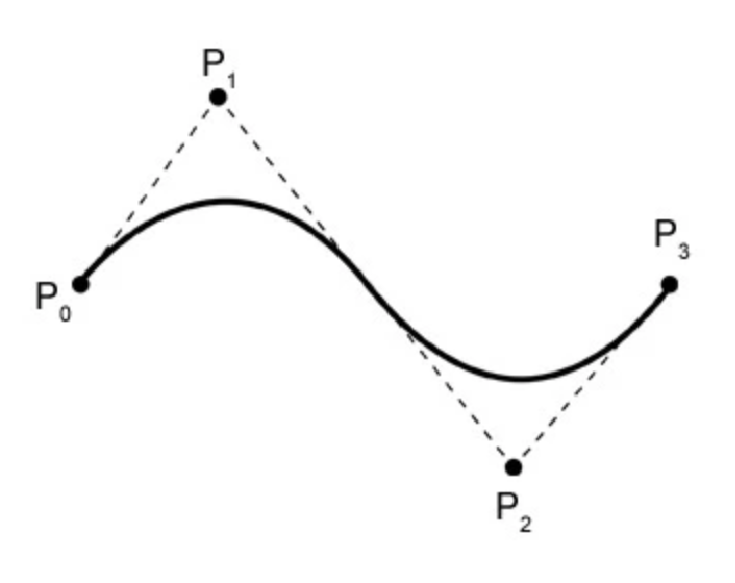
\includegraphics[width=0.3\textwidth]{cubic_bezier_curve.eps}
    \caption{The cubic Bezier curve.}
    \label{f:cubic_bezier_curve}
\end{figure}
% figure downloaded from: https://btnseniorproject17.wordpress.com/2017/05/01/more-unity-part-2-path-following-and-bezier-curves/

The items of Bernstein basis polynomials of degree $n$ are defined as
\begin{equation}
    b_{m, n}(t) = {n \choose m} t^m (1-t)^{n-m}
    \label{e:cbc:bbp}
\end{equation}
where ${n \choose m}$ is a binomial coefficient and $m = 0, 1, \dots, n$. The Bernstein basis polynomials have the
following properties:
\begin{enumerate}
    \item
    $b_{m, n}(t) = 0$, if $m<0$ or $m>n$.
    \item
    $b_{m, n}(t) \geq 0$, for $t \in [0, 1]$.
    \item
    $b_{m, n}(1-t) = b_{n-m, n}(t)$.
\end{enumerate}
The cubic Bezier curve is defined by 4 control points $\mathbf{P}_i$, $i = 0, 1, 2, 3$:
\begin{equation*}
    \mathbf{P}_i =
    \begin{bmatrix}
        P_{xi} \\ P_{yi}
    \end{bmatrix}
\end{equation*}
The function $\mathbf{B}(t)$ is
\begin{equation*}
    \mathbf{B}(t) = \Sigma b_{i,3}(t)\mathbf{P}_i
\end{equation*}
where $b_{i,3}(t)$ is shown in Eq.~(\ref{e:cbc:bbp}). This function can be expanded to
\begin{equation}
    \mathbf{B}(t) = (1-t)^3 \mathbf{P}_0 + 3(1-t)^2 t \mathbf{P}_1 + 3(1-t) t^2 \mathbf{P}_2 + t^3 \mathbf{P}_3
    \label{e:cbc:der0}
\end{equation}
where $0 \leq t \leq 1$.  The first-order derivative of $\mathbf{B}(t)$ is
\begin{equation*}
    \mathbf{B}^\prime(t) = 3 \left[
        (1-t)^2 (\mathbf{P}_1 - \mathbf{P}_0) +
        2(1-t)t(\mathbf{P}_2 - \mathbf{P}_1) +
        t^2(\mathbf{P}_3 - \mathbf{P}_2) \right]
\end{equation*}
The second-order derivative of $B(t)$ is
\begin{equation*}
    \mathbf{B}^{\prime \prime}(t) = 6 \left[
        (1-t)(\mathbf{P}_2 - 2\mathbf{P}_1 +\mathbf{P}_0) +
        t(\mathbf{P}_3 - 2\mathbf{P}_2 + \mathbf{P}_1) \right]
\end{equation*}

For a sequence of $n$ cubic Bezier curves, $\mathbf{B}_0(t)$ through $\mathbf{B}_{n-1}(t)$, there are $4n$ control
points can be adjusted. It implies that there are $4n$ dimensions of freedom. Assume the first and last points are fixed.
If we wish the value, slope, and curvature between any two Bezier curves are continuous, the degree of freedom will
become $n+1$. Thus, we can keep the continuous value of curvature when adding the number of Bezier curves.